% \def\axisdefaultticklabel{$\pgfmathprintnumber{\tick}$}

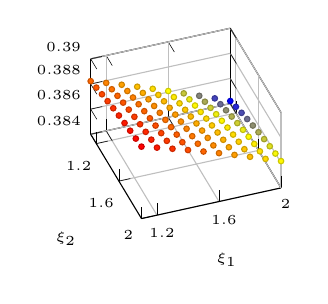
\begin{tikzpicture}
 
\begin{axis}[
% hide x axis,
% hide y axis,
% tick align=outside,
view/h=70,
view/v=50,
tick pos=left,
% x grid style={darkgray176},
% xlabel style={rotate=-10},
xlabel={\(\displaystyle \xi_2\)},
xtick = {1.2,1.6,2},
% xmin=1.0395, xmax=1.1605,
xtick style={color=black},
% y grid style={darkgray176},
% ylabel style={rotate=45},
ylabel={\(\displaystyle \xi_1\)},
ytick = {1.2,1.6,2},
% ymin=1.0395, ymax=1.1605,
ytick style={color=black},
% yticklabel style={anchor=center}
% zticklabels = {0.387,0.389,0.39, 0.392},
z tick label style={/pgf/number format/precision=3},
zmin=0.384, zmax=0.39,
ztick style={color=black},
width=4cm,height=4cm,
font = \tiny, 
grid
]
 
\addplot3[
  mark=*,
  mark size=1pt,
  only marks,
  scatter,
  scatter/@post marker code/.code={%
  \endscope
},
%   scatter/@pre marker code/.code={%
%   \expanded{%
%   \noexpand\definecolor{thispointdrawcolor}{RGB}{\drawcolor}%
%   \noexpand\definecolor{thispointfillcolor}{RGB}{\fillcolor}%
%   }%
%   \scope[draw=thispointdrawcolor, fill=thispointfillcolor]%
% },
%   visualization depends on={value \thisrow{draw} \as \drawcolor},
%   visualization depends on={value \thisrow{fill} \as \fillcolor}
] table 
{
% x y   z
% 1.1 1.1   0.39946797
% 1.1 1.2 0.40073798
% }
x    y         z
1.1	1.1	0.38822708
1.1	1.2	0.3878177 
1.1	1.3	0.3873986 
1.1	1.4	0.38696966
1.1	1.5	0.38653117
1.1	1.6	0.38608363
1.1	1.7	0.38562652
1.1	1.8	0.38516018
1.1	1.9	0.38468498
1.1	2.0	0.384201  
1.2	1.1	0.38845968
1.2	1.2	0.38805744
1.2	1.3	0.38764504
1.2	1.4	0.3872227 
1.2	1.5	0.38679066
1.2	1.6	0.38634878
1.2	1.7	0.38589743
1.2	1.8	0.3854364 
1.2	1.9	0.3849663 
1.2	2.0	0.38448724
1.3	1.1	0.3886749 
1.3	1.2	0.38827953
1.3	1.3	0.3878741 
1.3	1.4	0.3874583 
1.3	1.5	0.38703215
1.3	1.6	0.38659596
1.3	1.7	0.38615018
1.3	1.8	0.38569444
1.3	1.9	0.38522935
1.3	2.0	0.3847548 
1.4	1.1	0.3888729 
1.4	1.2	0.3884847 
1.4	1.3	0.38808578
1.4	1.4	0.38767618
1.4	1.5	0.38725623
1.4	1.6	0.3868259 
1.4	1.7	0.38638523
1.4	1.8	0.3859346 
1.4	1.9	0.38547435
1.4	2.0	0.38500416
1.5	1.1	0.38905445
1.5	1.2	0.38867337
1.5	1.3	0.3882807 
1.5	1.4	0.38787726
1.5	1.5	0.3874631 
1.5	1.6	0.3870382 
1.5	1.7	0.38660288
1.5	1.8	0.3861572 
1.5	1.9	0.38570136
1.5	2.0	0.3852356 
1.6	1.1	0.3892199 
1.6	1.2	0.38884515
1.6	1.3	0.3884591 
1.6	1.4	0.38806176
1.6	1.5	0.38765323
1.6	1.6	0.38723376
1.6	1.7	0.38680342
1.6	1.8	0.38636228
1.6	1.9	0.38591096
1.6	2.0	0.3854493 
1.7	1.1	0.38936958
1.7	1.2	0.38900158
1.7	1.3	0.38862154
1.7	1.4	0.38823003
1.7	1.5	0.387827  
1.7	1.6	0.38741255
1.7	1.7	0.38698718
1.7	1.8	0.3865506 
1.7	1.9	0.38610354
1.7	2.0	0.38564584
1.8	1.1	0.38950405
1.8	1.2	0.3891423 
1.8	1.3	0.38876835
1.8	1.4	0.3883825 
1.8	1.5	0.3879847 
1.8	1.6	0.38757548
1.8	1.7	0.3871547 
1.8	1.8	0.38672248
1.8	1.9	0.38627943
1.8	2.0	0.3858254 
1.9	1.1	0.38962328
1.9	1.2	0.38926792
1.9	1.3	0.3888999 
1.9	1.4	0.38851953
1.9	1.5	0.38812703
1.9	1.6	0.38772246
1.9	1.7	0.38730612
1.9	1.8	0.38687834
1.9	1.9	0.38643894
1.9	2.0	0.3859885 
2.0	1.1	0.38972837
2.0	1.2	0.38937902
2.0	1.3	0.38901663
2.0	1.4	0.3886415 
2.0	1.5	0.38825408
2.0	1.6	0.38785404
2.0	1.7	0.38744193
2.0	1.8	0.38701817
2.0	1.9	0.3865824 
2.0	2.0	0.38613522
};
\end{axis}
 
\end{tikzpicture}

